\newpage
\section{Opis proponowanego rozwiązania}
Proponujemy rozwiązanie oparte na artykule „Convolutional Neural Networks for Sentence
Classification”\cite{cnn}. Sieć zaczyna się od warstwy embeddingowej dostarczajączej
wektory słów. Po niej następuje przetwarzanie przez blok konwolucyjny składający się z jednowymiarowych warstw
splotowych, których wielkość kernela będzie zależała od tego, jakie n-gramy będzie analizować
, tzn. wielkość kernela odpowiada wielkości n-gramu. Warstwy konwolucyjne będą zakończone
funkcją aktywacji ReLU. Blok może składać się z wielu warstw -- określenie ilości 
analizowanych n-gramów będzie pozostawione użytkownikowi sieci.
Po splocie następuje warstwa poolingowa realizująca
max-over-time pooling. Ostatni blok sieci stanowi warstwa gęsta z warstwą dropout
(w celach regularyzacji), zakończony jest softmaxem.

Jako optymalizator zostanie zastosowany Adam, zaś funkcją kosztu z racji wieloklasowości
problemu będzie entropia skrośna.

\begin{figure}[h!]
    \centering
        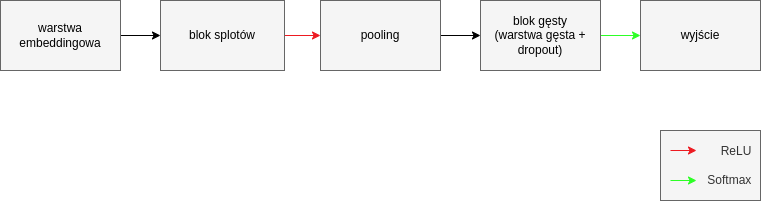
\includegraphics[width=0.8\linewidth]{img/architecture.png}
    \caption{Proponowana architektura klasyfikatora opartego warstwach splotowych.}
\end{figure}

Drugi model do celów porównawczych będzie oparty o wektor słów z pretrenowanego modelu
transformatorowego BERT\cite{bert}. Zmiana tyczy się tylko warstwy embeddingowej -- będą do niej
wprowadzone inne wektory.
